% Module 1: What This Is and What You Can Do With It
% Beamer Presentation — Claude Code for Academic Researchers
\documentclass[aspectratio=169, 11pt]{beamer}

% ── Theme and Colors ──────────────────────────────────────────────
\usetheme{Madrid}
\usecolortheme{default}

% Custom colors
\definecolor{anthropic}{RGB}{50, 50, 80}
\definecolor{accent}{RGB}{180, 90, 40}
\definecolor{lightgray}{RGB}{245, 245, 245}

\setbeamercolor{structure}{fg=anthropic}
\setbeamercolor{frametitle}{bg=anthropic, fg=white}
\setbeamercolor{title}{bg=anthropic, fg=white}
\setbeamercolor{block title}{bg=anthropic, fg=white}
\setbeamercolor{block body}{bg=lightgray}
\setbeamercolor{alerted text}{fg=accent}

\setbeamerfont{title}{size=\Large, series=\bfseries}
\setbeamerfont{frametitle}{size=\large, series=\bfseries}

% ── Packages ──────────────────────────────────────────────────────
\usepackage{graphicx}
\usepackage{booktabs}
\usepackage{listings}
\usepackage{fontenc}
\usepackage{hyperref}
\usepackage{tikz}

\lstset{
  basicstyle=\ttfamily\small,
  backgroundcolor=\color{lightgray},
  frame=single,
  framerule=0pt,
  breaklines=true,
  columns=fullflexible,
}

% ── Metadata ──────────────────────────────────────────────────────
\title{Module 1: What This Is and What You Can Do With It}
\subtitle{Claude Code for Academic Researchers}
\author{} % Instructor name
\date{}
\institute{}

% ══════════════════════════════════════════════════════════════════
\begin{document}

% ── Title ─────────────────────────────────────────────────────────
\begin{frame}[plain]
  \titlepage
\end{frame}

% ══════════════════════════════════════════════════════════════════
%  OPENING DEMO  [0:00–2:00]
% ══════════════════════════════════════════════════════════════════

\begin{frame}{Live Demo: The Data}
  \textbf{Dataset 1: County Presidential Election Returns}
  \begin{itemize}
    \item Source: MIT Election Data + Science Lab
    \item County-level vote totals by candidate and party, 2000--2024
    \item ${\sim}$94{,}000 rows --- one row per county $\times$ year $\times$ candidate
    \item Variables: FIPS codes, candidate names, party, vote counts, vote mode
  \end{itemize}

  \vspace{0.5em}
  \textbf{Dataset 2: IPUMS American Community Survey Microdata}
  \begin{itemize}
    \item Source: IPUMS USA (University of Minnesota)
    \item Person-level survey records with demographic, economic, and geographic variables
    \item ${\sim}$15 million rows per year --- one row per person
    \item Variables: age, education, employment, income, race, poverty status, county FIPS
  \end{itemize}
\end{frame}

\begin{frame}{Live Demo: The Task}
  \textbf{Goal:} Build a county-year panel joining election results with demographics.

  \vspace{0.5em}
  This requires:
  \begin{enumerate}
    \item Reshape election data to one row per county-year with vote shares
    \item Aggregate 15M person-level records to county-level means using survey weights
    \item Harmonize FIPS codes across datasets (different formats)
    \item Merge on county $\times$ year and validate the join
  \end{enumerate}

  \vspace{0.5em}
  In Stata or R, this takes 30--45 minutes of careful coding.

  {\footnotesize\textit{[Switch to terminal]}}
\end{frame}

% ══════════════════════════════════════════════════════════════════
%  WHAT JUST HAPPENED  [2:00–10:00]
% ══════════════════════════════════════════════════════════════════

\begin{frame}{What Just Happened}
  \begin{columns}[T]
    \begin{column}{0.48\textwidth}
      \textbf{It wrote the code:}
      \begin{itemize}
        \item Read both files
        \item Identified the join key
        \item Handled cleaning steps
        \item Wrote a complete script
      \end{itemize}
    \end{column}
    \begin{column}{0.48\textwidth}
      \textbf{It also:}
      \begin{itemize}
        \item Understood the data structure\\
          {\small (person-level vs.\ county-level,\\survey weights, FIPS formats)}
        \item Ran the code and diagnosed errors
        \item Provided summaries of the output\\
          {\small (row counts, variable descriptions,\\merge diagnostics)}
      \end{itemize}
    \end{column}
  \end{columns}

  \vspace{0.5em}
  \alert{But it also made a decision about our data without asking.}

  \vspace{0.5em}
  Both of these things are true:
  \begin{enumerate}
    \item It took 90 seconds instead of 45 minutes
    \item It made analytical choices autonomously
  \end{enumerate}
\end{frame}

\begin{frame}{The RA Analogy}
  \begin{block}{How to Think About Claude Code}
    Claude Code is like a research assistant who is:
    \begin{itemize}
      \item Extremely fast
      \item Has read a lot
      \item Will \textbf{never} say ``I don't know how to do that''
    \end{itemize}
    \vspace{0.3em}
    Instead, it will just do it wrong and hand it in.
  \end{block}

  \vspace{0.5em}
  You have all managed RAs. You know how valuable---and how dangerous---that profile is.

  \vspace{0.5em}
  \textbf{This course teaches you to capture the value while managing the risk.}
\end{frame}

% ══════════════════════════════════════════════════════════════════
%  THE CODING PARADIGM SPECTRUM  [10:00–16:00]
% ══════════════════════════════════════════════════════════════════

\begin{frame}{The Coding Paradigm Spectrum}
  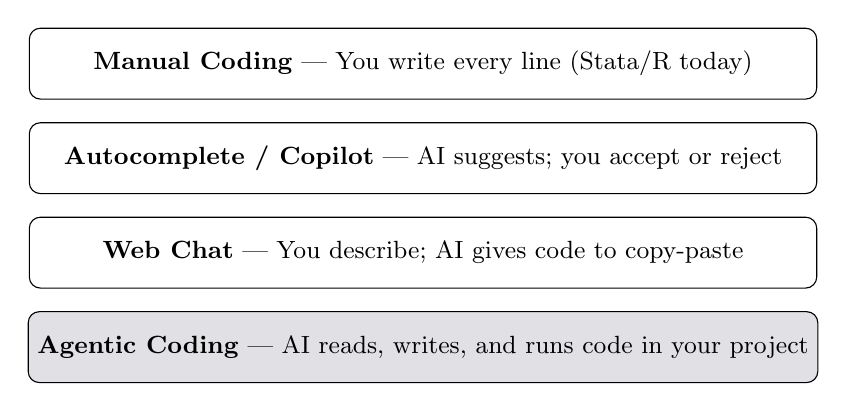
\begin{tikzpicture}[
    node distance=0.3cm,
    every node/.style={draw, rounded corners, minimum width=10cm, minimum height=0.9cm, align=center, font=\small},
    arrow/.style={->, thick, >=stealth}
  ]
    \node (manual) at (0,3.6) {\textbf{Manual Coding} --- You write every line (Stata/R today)};
    \node (copilot) at (0,2.4) {\textbf{Autocomplete / Copilot} --- AI suggests; you accept or reject};
    \node (chat) at (0,1.2) {\textbf{Web Chat} --- You describe; AI gives code to copy-paste};
    \node[fill=anthropic!15] (agentic) at (0,0) {\textbf{Agentic Coding} --- AI reads, writes, and runs code in your project};
  \end{tikzpicture}

  \vspace{0.5em}
  \centering
  \small $\uparrow$ More autonomy, more power, more risk $\uparrow$
\end{frame}

\begin{frame}{Why Agentic Coding Is Different}
  \begin{alertblock}{The Key Insight}
    Agentic coding is the first paradigm where the tool \textbf{modifies your project directly}.
  \end{alertblock}

  \vspace{0.5em}
  That is what makes it so productive---and why learning to use it well matters.

  \vspace{0.5em}
  These principles apply to Claude Code, Cursor, Windsurf, or whatever comes next.
\end{frame}

% ══════════════════════════════════════════════════════════════════
%  WHAT IT CAN AND CANNOT DO  [16:00–19:00]
% ══════════════════════════════════════════════════════════════════

\begin{frame}{What Claude Code Can Do}
  \begin{columns}[T]
    \begin{column}{0.48\textwidth}
      \textbf{Delegate freely:}
      \begin{itemize}
        \item Write code rapidly
        \item Clean data
        \item Generate robustness checks
        \item Create visualizations
      \end{itemize}
    \end{column}
    \begin{column}{0.48\textwidth}
      \textbf{Delegate freely (cont.):}
      \begin{itemize}
        \item Audit existing code
        \item Write documentation
        \item Build replication packages
        \item Process text at scale
      \end{itemize}
    \end{column}
  \end{columns}
\end{frame}

\begin{frame}{What Requires Human Judgment}
  \begin{block}{The Referee Test}
    If a referee questioned this choice, who would need to answer---you or the RA?
  \end{block}

  \vspace{0.5em}
  \textbf{Do not delegate:}
  \begin{itemize}
    \item Choosing specifications
    \item Interpreting results
    \item Identification strategies
    \item Sample selection decisions
  \end{itemize}
\end{frame}

% ══════════════════════════════════════════════════════════════════
%  WHY VERIFICATION MATTERS  [19:00–23:00]
% ══════════════════════════════════════════════════════════════════

\begin{frame}{Why Verification Matters}
  {\large What happens when you skip verification:}

  \vspace{0.8em}
  \begin{enumerate}
    \item \textbf{Silent observation loss:} A merge silently drops 300 observations.\\
      The code looks clean. The error is invisible without checking row counts.

      \vspace{0.5em}
    \item \textbf{Invalid transformation:} A log transformation applied to a variable containing zeros.\\
      No error raised, wrong results.

      \vspace{0.5em}
    \item \textbf{Incorrect panel operations:} A lagged variable computed without sorting by time within panels.
  \end{enumerate}

  \vspace{0.5em}
  \alert{These are the kinds of errors that end up in published work.}
\end{frame}

% ══════════════════════════════════════════════════════════════════
%  THE CONTROL PRINCIPLE  [23:00–25:00]
% ══════════════════════════════════════════════════════════════════

\begin{frame}{The Control Principle}
  \begin{alertblock}{You Are the PI. Claude Code Is the RA.}
    The question is not ``can Claude Code do this'' but\\
    ``what is the best way to get this done reliably.''
  \end{alertblock}

  \vspace{1em}
  \centering
  \textbf{If you cannot verify a result, you should not delegate the task.}

  \vspace{1em}
  That is the standard we hold ourselves to today.
\end{frame}

% ══════════════════════════════════════════════════════════════════
%  WHY PYTHON  [25:00–27:00]
% ══════════════════════════════════════════════════════════════════

\begin{frame}{Why Python}
  \begin{itemize}
    \item Claude Code is substantially better at Python than Stata or R
    \item The principles---task decomposition, verification, control---transfer to any language
    \item Python is increasingly where the tools and ecosystem are for computational research
  \end{itemize}
\end{frame}

% ══════════════════════════════════════════════════════════════════
%  SETUP  [27:00–37:00]
% ══════════════════════════════════════════════════════════════════

\begin{frame}{Setup Check}
  \begin{enumerate}
    \item Open your terminal
    \item Verify Node.js: \lstinline{node --version}
    \item Verify Claude Code: \lstinline{claude --version}
    \item Authenticate: \lstinline{claude}
  \end{enumerate}

  \vspace{1em}
  \textbf{If you completed pre-work:} help your neighbor.\\
  \textbf{If you're stuck:} pair with someone who is set up---we'll troubleshoot at break.
\end{frame}

% ══════════════════════════════════════════════════════════════════
%  EXERCISE  [37:00–47:00]
% ══════════════════════════════════════════════════════════════════

\begin{frame}{Exercise: Your First Commands}
  \textbf{Task 1} (low-stakes):\\
  Here is a Python script that cleans a dataset.\\
  Ask Claude Code to explain what it does, line by line.

  \vspace{0.8em}
  \textbf{Task 2} (introduces verification):\\
  Ask Claude Code to add an assertion that the row count after cleaning matches the expected count.

  \vspace{0.8em}
  \textbf{Stretch:}\\
  Ask Claude Code to handle a new edge case---negative values in a column that should be positive.
\end{frame}

\begin{frame}{Exercise Debrief}
  \begin{itemize}
    \item What did it get right?
    \item Anything wrong or confusing?
    \item That is normal and expected
  \end{itemize}
\end{frame}

% ══════════════════════════════════════════════════════════════════
%  PREVIEW  [47:00–50:00]
% ══════════════════════════════════════════════════════════════════

\begin{frame}{What's Ahead Today}
  By the end of the day, you will have:
  \begin{itemize}
    \item Built a documented data pipeline
    \item Generated robustness checks
    \item Audited code for errors
    \item Learned version control for agent-assisted work
  \end{itemize}

  \vspace{0.5em}
  You will know which parts Claude Code should handle and which require your judgment.

  \vspace{0.5em}
  \textbf{And you will be able to take these workflows back to your own research.}
\end{frame}

\end{document}
